\documentclass[12pt]{beamer}

\usepackage[utf8]{inputenc}
\usepackage[T1]{fontenc}
\usepackage[english]{babel}
\usepackage{amsmath}
\usepackage{amssymb}
\usepackage{pgfornament}
\usepackage{amsthm}
\usepackage{stmaryrd} %for \llbracket and \rrbracket
%\usepackage{bbold} %for a nice \mathbb{1}
\usepackage{graphicx}
\usepackage{float}
\usepackage{bbm}
\usepackage{arcs}
\usepackage{calc}
\renewcommand{\mathbb}[1]{\mathbbm{#1}}

\everymath{\displaystyle}

\usepackage[
  leftmargin = 0pt,
  innerleftmargin = 1em,
  innertopmargin = 0pt,
  innerbottommargin = 0pt,
  innerrightmargin = 0pt,
  rightmargin = 0pt,
  linewidth = 3pt,
  topline = false,
  rightline = false,
  bottomline = false,
]{mdframed}

\newcommand{\floor}[1]{\lfloor #1 \rfloor}
\newcommand{\ceil}[1]{\lceil #1 \rceil}
\newcommand{\eps}{\varepsilon} % j'aime pas "eps"
\renewcommand{\epsilon}{\varepsilon}
\renewcommand{\phi}{\varphi}

\newcommand{\dd}{\mathrm{d}}
\newcommand{\der}[2]{\frac{\dd #1}{\dd #2}}
\newcommand{\dern}[3]{\frac{\dd^{#3} #1}{\dd {#2}^{#3}}}
\newcommand{\dpar}[2]{\frac{\partial #1}{\partial #2}}
\newcommand{\dparn}[3]{\frac{\partial^{#3} #1}{\partial {#2}^{#3}}}
\newcommand{\infsum}{\sum^{+\infty}}
\newcommand{\infprod}{\prod^{+\infty}}

\newcommand{\sep}{\begin{center} \pgfornament[width=10cm]{88} \end{center}}
\newcommand{\finish}{\begin{center} \pgfornament[width=5cm]{75} \end{center}}
\DeclareMathOperator{\id}{id}


%\linespread{1.1}
%\setlength{\parskip}{1em plus2mm minus2mm}


%  _____ _
% |_   _| |__   ___  ___  _ __ ___ _ __ ___  ___
%   | | | '_ \ / _ \/ _ \| '__/ _ \ '_ ` _ \/ __|
%   | | | | | |  __/ (_) | | |  __/ | | | | \__ \
%   |_| |_| |_|\___|\___/|_|  \___|_| |_| |_|___/

\newtheoremstyle{defistyle}{}{}{\normalfont}{}{\bfseries}{\ :}{ }{}
\newtheoremstyle{theostyle}{}{}{\normalfont}{}{\bfseries}{}{ }{}
\newtheoremstyle{axiostyle}{}{}{\normalfont}{}{\bfseries}{}{ }{}
\newtheoremstyle{preuvestyle}{}{}{\normalfont}{}{\normalfont}{\ :}{ }{}

\definecolor{emerald}{rgb}{0.31, 0.78, 0.47}
\newmdenv[
  linecolor = emerald!100
]{leftbargreen}

\definecolor{seablue}{rgb}{0.0, 0.412, 0.58}
\newmdenv[
  linecolor = seablue!100
]{leftbarblue}

\definecolor{orange}{rgb}{1.0, 0.6, 0.0}
\newmdenv[
  linecolor = orange!100
]{leftbarorange}

\definecolor{red}{rgb}{0.9, 0.0, 0.0}
\newmdenv[
  linecolor = red!100
]{leftbarred}

\definecolor{violet}{rgb}{0.58, 0.0, 0.83}
\newmdenv[
  linecolor = violet!100
]{leftbarviolet}

\definecolor{brown}{rgb}{0.59, 0.29, 0.0}
\newmdenv[
  linecolor = brown!100
]{leftbarbrown}

\theoremstyle{defistyle}
\newtheorem{definth}{Définition}[section]
\theoremstyle{theostyle}
\newtheorem{theonth}{Th\'eor\`eme}[subsection]
\newtheorem*{propnth}{Propriété}
\newtheorem*{propsnth}{Propriétés}
\newtheorem{proponth}[theonth]{Proposition}
\newtheorem{cornth}[theonth]{Corollaire}
\newtheorem{lemnth}[theonth]{Lemme}
\newtheorem*{exnth}{Exemple}
\newtheorem*{exsnth}{Exemples}
\theoremstyle{preuvestyle}
\newtheorem*{remnth}{Remarque}
\newtheorem*{remsnth}{Remarques}
\newtheorem*{pvnth}{Démonstration}
\theoremstyle{axiostyle}
\newtheorem*{axinth}{Axiome}
\newtheorem*{lointh}{Loi}
\newtheorem*{postnth}{Postulat}

\newenvironment{defi}[1]
  {\begin{leftbarred}\begin{definth} \textbf{#1}\ \\}
  {\end{definth}\end{leftbarred}}
\newenvironment{prop}[1][]
  {\begin{leftbarviolet}\begin{proponth} \textbf{#1}\ \\}
  {\end{proponth}\end{leftbarviolet}}
\newenvironment{props}[1][]
  {\begin{leftbarviolet}\begin{propsnth} \textbf{#1} \begin{enumerate}}
  {\end{enumerate}\end{propsnth}\end{leftbarviolet}}
\newenvironment{propo}[1][]
  {\begin{leftbarviolet}\begin{proponth} \textbf{#1}\  \\}
  {\end{proponth}\end{leftbarviolet}}
\newenvironment{theo}[1]
  {\begin{leftbarviolet}\begin{theonth} \textbf{#1}\ \\}
  {\end{theonth}\end{leftbarviolet}}
\newenvironment{cor}[1][]
  {\begin{leftbarviolet}\begin{cornth} \textbf{#1}\ \\}
  {\end{cornth}\end{leftbarviolet}}
\newenvironment{lem}[1][]
  {\begin{leftbarviolet}\begin{lemnth} \textbf{#1}\ \\}
  {\end{lemnth}\end{leftbarviolet}}
\newenvironment{ex}[1][]
  {\begin{leftbarorange}\begin{exnth} \textbf{#1}\ \\}
  {\end{exnth}\end{leftbarorange}}
\newenvironment{exs}[1][]
  {\begin{leftbarorange}\begin{exsnth} \textbf{#1}\begin{enumerate}}
  {\end{enumerate}\end{exsnth}\end{leftbarorange}}
\newenvironment{rem}
  {\begin{leftbarbrown}\begin{remnth}}
  {\end{remnth}\end{leftbarbrown}}
\newenvironment{rems}
  {\begin{leftbarbrown}\begin{remnth}\begin{itemize}}
  {\end{itemize}\end{remnth}\end{leftbarbrown}}
\newenvironment{pv}
  {\begin{leftbargreen}\begin{pvnth}}
  {\hfill$\square$\end{pvnth}\end{leftbargreen}}
\newenvironment{axi}[1][]
  {\begin{leftbarblue}\begin{axinth} \textbf{#1}\ \\}
  {\end{axinth}\end{leftbarblue}}
\newenvironment{loi}[1][]
  {\begin{leftbarblue}\begin{lointh} \textbf{#1}\ \\}
  {\end{lointh}\end{leftbarblue}}
\newenvironment{post}[1][]
  {\begin{leftbarblue}\begin{postnth} \textbf{#1}\ \\}
  {\end{postnth}\end{leftbarblue}}


%   ____                           _                   _   _
%  / ___| ___ _ __   ___ _ __ __ _| |  _ __ ___   __ _| |_| |__  ___
% | |  _ / _ \ '_ \ / _ \ '__/ _` | | | '_ ` _ \ / _` | __| '_ \/ __|
% | |_| |  __/ | | |  __/ | | (_| | | | | | | | | (_| | |_| | | \__ \
%  \____|\___|_| |_|\___|_|  \__,_|_| |_| |_| |_|\__,_|\__|_| |_|___/


\renewcommand{\le}{\leqslant}
\renewcommand{\ge}{\geqslant}

\newcommand{\R}{\ensuremath{\mathbb{R}}}
\newcommand{\Rb}{\ensuremath{\overline{\mathbb{R}}}}
\newcommand{\N}{\ensuremath{\mathbb{N}}}
\newcommand{\Q}{\ensuremath{\mathbb{Q}}}
\newcommand{\Z}{\ensuremath{\mathbb{Z}}}
\newcommand{\C}{\ensuremath{\mathbb{C}}}
\newcommand{\U}{\ensuremath{\mathbb{U}}}
\newcommand{\F}{\ensuremath{\mathbb{F}}}
\newcommand{\K}{\ensuremath{\mathbb{K}}}

\newcommand{\imp}{\;\Rightarrow\;}
\newcommand{\pmi}{\;\Leftarrow\;}
\newcommand{\eq}{\;\Leftrightarrow\;}
\newcommand{\tq}{\;|\;}

\newcommand{\et}{\text{ et }}
\newcommand{\ou}{\text{ ou }}
\newcommand{\si}{\text{ si }}
\newcommand{\sinon}{\text{ sinon }}

\newcommand{\eint}[1]{\llbracket #1 \rrbracket}

\newcommand{\app}[3][0cm]{\hspace{-#1} \mbox{\raisebox{#2}{$\begin{aligned}#3
\end{aligned}$}} }
%auto app
\newcommand{\aapp}[2][0cm]{\hspace{-#1} \mbox{\raisebox{- \height+2ex}{$\begin{aligned}#2
\end{aligned}$}} }




\usepackage{mathrsfs}
\usetikzlibrary{positioning,calc}
\usepackage{tikz-cd}
\usepackage{ebproof}
\newcommand\M{\text{M}(X\uplus X^{-1})}
\newcommand\G{\mathscr{G}(X)}
\renewcommand\F{\mathscr{F}(X)}
\newcommand\V{\mathbb{V}}
\newcommand\E{\mathbb{E}}
\newcommand\D{\mathbb{D}}
\newcommand\bet{\rightarrow_\beta}
\newcommand\beq{=_\beta}
\newcommand\Rel{\text{Rel}}
\newcommand\Set{\text{Set}}
\newcommand\Oper{\text{Oper}}
\newcommand\Inv{\text{Inv}}
\newcommand\Pol{\text{Pol}}
\renewcommand\P{\mathscr{P}}
\newcommand\ar{\text{ar}}
\newcommand\arf{\text{ar}}
\newcommand\csp{\text{CSP}}
\renewcommand\C{\mathscr{C}}
\newcommand\fset{\text{FinSet}}
\newcommand\ffun{\text{FinFun}}
\newcommand\im{\text{Im }}
\newcommand\sem[1]{\llbracket {#1} \rrbracket}
\newcommand\ext{\text{Ext}}
\newcommand\fns{\mathscr{F}}
\newcommand\brk[1]{[ {#1} ]}
\newcommand\psh{\text{PSh}}
\newcommand\sh{\text{Sh}}
\newcommand\shc{\text{Sh}_\text{can}}
\newcommand{\tproof}[1]{{\scantokens{\begin{prooftree}#1\end{prooftree}}}}
\newcommand{\cf}{\mathbb{F}}
\newcommand{\tsigma}{\widetilde{\Sigma}}
\newcommand{\tgamma}{\widetilde{\Gamma}}
\newcommand{\tlambda}{\widetilde{\Lambda}}
\newcommand{\colim}{\text{colim}}
\newcommand{\fcsp}{\text{FCSP}}
\newcommand{\op}{\text{op}}
\newcommand{\tf}{\widetilde{F}}
\newcommand{\tg}{\widetilde{G}}
\newcommand{\tH}{\widetilde{H}}
\newcommand{\ml}[1]{\langle{#1}\rangle}


%  ____                                    ____             __ _       
% | __ )  ___  __ _ _ __ ___   ___ _ __   / ___|___  _ __  / _(_) __ _ 
% |  _ \ / _ \/ _` | '_ ` _ \ / _ \ '__| | |   / _ \| '_ \| |_| |/ _` |
% | |_) |  __/ (_| | | | | | |  __/ |    | |__| (_) | | | |  _| | (_| |
% |____/ \___|\__,_|_| |_| |_|\___|_|     \____\___/|_| |_|_| |_|\__, |
%                                                                |___/ 
\usepackage{etoolbox}
\makeatletter
\preto{\@verbatim}{\topsep=0pt \partopsep=0pt }
\makeatother

% Le logo
\logo{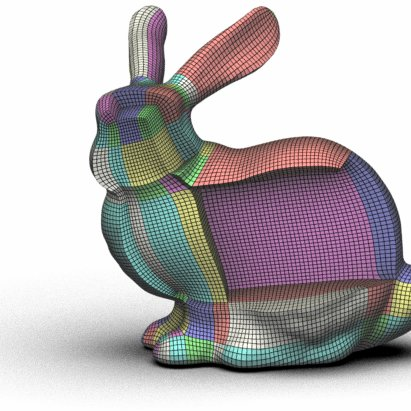
\includegraphics[scale=0.07]{logo.jpg}}

% Au début de chaque section
\AtBeginSection[]{
	\begin{frame}
		\frametitle{\textbf{\insertsectionhead}}
        \framesubtitle{Section \thesection}
		\tableofcontents[currentsection,hideothersubsections]
	\end{frame}
}

% Au début de chaque sous-section
\AtBeginSubsection[]{
	\begin{frame}
        \frametitle{\textbf{Section} \thesection-\thesubsection}
        \begin{block}{Subsection \thesubsection}
			\Large \textbf{\insertsubsectionhead}
		\end{block}
	\end{frame}
}

%Put a nice theme
\usetheme{Berkeley}
\beamertemplatenavigationsymbolsempty
\makeatletter
\g@addto@macro\scriptsize{%
\setlength\abovedisplayskip{1pt}
\setlength\belowdisplayskip{1pt}
\setlength\abovedisplayshortskip{1pt}
\setlength\belowdisplayshortskip{1pt}
}
\g@addto@macro\normalsize{%
\setlength\abovedisplayskip{1pt}
\setlength\belowdisplayskip{1pt}
\setlength\abovedisplayshortskip{1pt}
\setlength\belowdisplayshortskip{1pt}
}
\makeatother
\setbeamertemplate{itemize item}[square]
\setbeamertemplate{itemize subitem}[triangle]

%  ____                                        _   
% |  _ \  ___   ___ _   _ _ __ ___   ___ _ __ | |_ 
% | | | |/ _ \ / __| | | | '_ ` _ \ / _ \ '_ \| __|
% | |_| | (_) | (__| |_| | | | | | |  __/ | | | |_ 
% |____/ \___/ \___|\__,_|_| |_| |_|\___|_| |_|\__|
%                                                  
\author{Antonin Reitz \and Luc Chabassier}
\title[Hex Mesh]
{Hexahedral Mesh Structure Visualization and Evaluation\\
    {\normalsize Paper presentation}}
\institute{\begin{center}MPRI
\end{center}}


\begin{document}
\addtobeamertemplate{block begin}{\setlength\abovedisplayskip{0pt}}

\begin{frame}
    \maketitle
\end{frame}

\begin{frame}
    \tableofcontents
\end{frame}

\section{Introduction}

\section{Definitions}

\begin{frame}[fragile]
  \frametitle{Hexagonal mesh}

  \begin{center}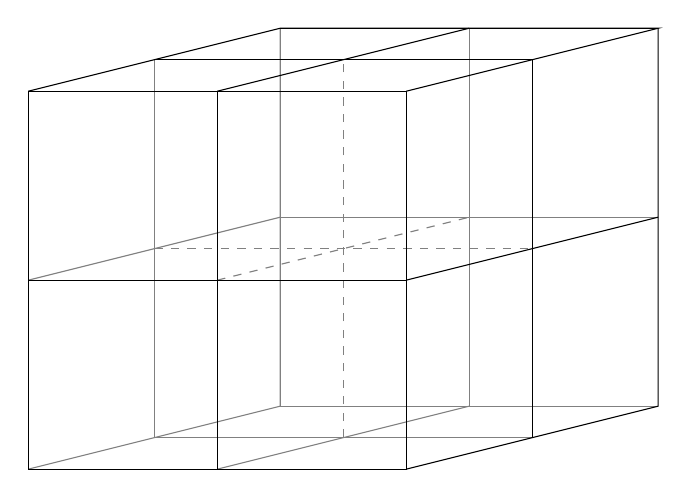
\begin{tikzpicture}[scale=0.8]
    \draw[color=gray] (0,0) -- (4,1) -- (4,7);
    \draw[color=gray] (4,1) -- (10,1);
    \draw[color=gray] (0,3) -- (4,4);
    \draw[color=gray] (2,0.5) -- (2,6.5);
    \draw[color=gray] (2,0.5) -- (8,0.5);
    \draw[color=gray] (3,0) -- (7,1);
    \draw[color=gray] (7,1) -- (7,7);
    \draw[color=gray] (4,4) -- (10,4);
    \draw[color=gray,dashed] (5,0.5) -- (5,6.5);
    \draw[color=gray,dashed] (2,3.5) -- (8,3.5);
    \draw[color=gray,dashed] (3,3) -- (7,4);

    \draw (0,0) -- (6,0) -- (6,6) -- (0,6) -- cycle;
    \draw (6,6) -- (10,7) -- (4,7) -- (0,6);
    \draw (6,0) -- (10,1) -- (10,7);
    \draw (3,0) -- (3,6);
    \draw (0,3) -- (6,3);
    \draw (8,0.5) -- (8,6.5);
    \draw (6,3) -- (10,4);
    \draw (3,6) -- (7,7);
    \draw (2,6.5) -- (8,6.5);
  \end{tikzpicture}\end{center}
\end{frame}

\begin{frame}[fragile]
  \frametitle{Basic vocabulary}

  \begin{center}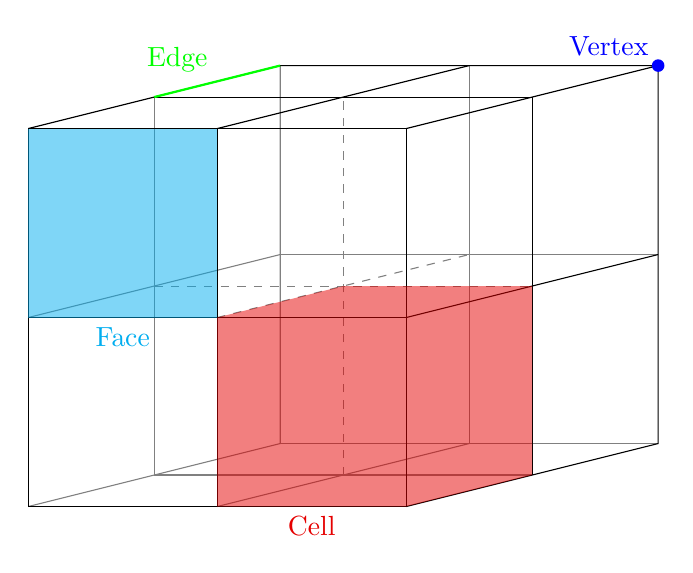
\begin{tikzpicture}[scale=0.8]
    \draw[color=gray] (0,0) -- (4,1) -- (4,7);
    \draw[color=gray] (4,1) -- (10,1);
    \draw[color=gray] (0,3) -- (4,4);
    \draw[color=gray] (2,0.5) -- (2,6.5);
    \draw[color=gray] (2,0.5) -- (8,0.5);
    \draw[color=gray] (3,0) -- (7,1);
    \draw[color=gray] (7,1) -- (7,7);
    \draw[color=gray] (4,4) -- (10,4);
    \draw[color=gray,dashed] (5,0.5) -- (5,6.5);
    \draw[color=gray,dashed] (2,3.5) -- (8,3.5);
    \draw[color=gray,dashed] (3,3) -- (7,4);

    \draw (0,0) -- (6,0) -- (6,6) -- (0,6) -- cycle;
    \draw (6,6) -- (10,7) -- (4,7) -- (0,6);
    \draw (6,0) -- (10,1) -- (10,7);
    \draw (3,0) -- (3,6);
    \draw (0,3) -- (6,3);
    \draw (8,0.5) -- (8,6.5);
    \draw (6,3) -- (10,4);
    \draw (3,6) -- (7,7);
    \draw (2,6.5) -- (8,6.5);

    \fill[color=blue,fill=blue] (10,7) circle (0.1);
    \node[anchor=south east,color=blue] at (10,7) {Vertex};
    \draw[thick,color=green] (2,6.5) -- (4,7);
    \node[anchor=south east,color=green] at (3,6.75) {Edge};
    \fill[color=cyan,fill=cyan,opacity=0.5] (0,6) -- (3,6) -- (3,3) -- (0,3) -- cycle;
    \node[anchor=north,color=cyan] at (1.5,3) {Face};
    \fill[color=red,fill=red,opacity=0.5] (3,0) -- (6,0) -- (8,0.5) -- (8,3.5) -- (5,3.5) -- (3,3) -- cycle;
    \node[anchor=north,color=red] at (4.5,0) {Cell};
  \end{tikzpicture}\end{center}
\end{frame}

\begin{frame}[fragile]
  \frametitle{Singularities}

  \begin{center}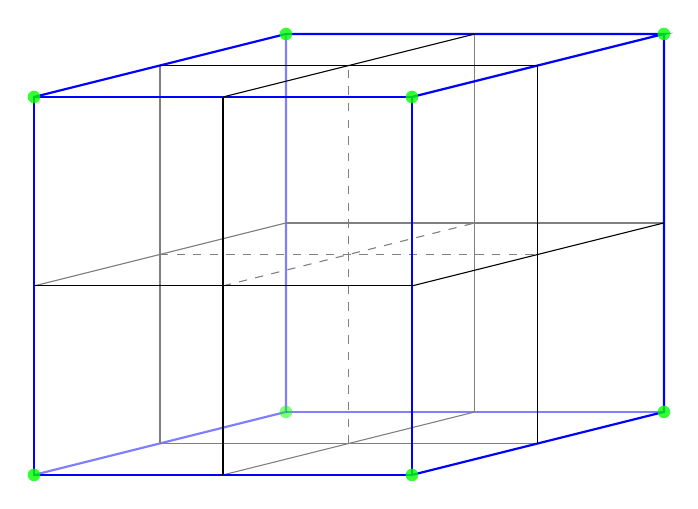
\begin{tikzpicture}[scale=0.8]
    \draw[thick,color=blue,opacity=0.5] (0,0) -- (4,1) -- (4,7);
    \draw[thick,color=blue,opacity=0.5] (4,1) -- (10,1);
    \draw[color=gray] (0,3) -- (4,4);
    \draw[color=gray] (2,0.5) -- (2,6.5);
    \draw[color=gray] (2,0.5) -- (8,0.5);
    \draw[color=gray] (3,0) -- (7,1);
    \draw[color=gray] (7,1) -- (7,7);
    \draw[color=gray] (4,4) -- (10,4);
    \draw[color=gray,dashed] (5,0.5) -- (5,6.5);
    \draw[color=gray,dashed] (2,3.5) -- (8,3.5);
    \draw[color=gray,dashed] (3,3) -- (7,4);

    \draw[thick,color=blue] (0,0) -- (6,0) -- (6,6) -- (0,6) -- cycle;
    \draw[thick,color=blue] (6,6) -- (10,7) -- (4,7) -- (0,6);
    \draw[thick,color=blue] (6,0) -- (10,1) -- (10,7);
    \draw (3,0) -- (3,6);
    \draw (0,3) -- (6,3);
    \draw (8,0.5) -- (8,6.5);
    \draw (6,3) -- (10,4);
    \draw (3,6) -- (7,7);
    \draw (2,6.5) -- (8,6.5);

    \fill[color=green,fill=green,opacity=0.8] (0,0) circle (0.1);
    \fill[color=green,fill=green,opacity=0.8] (6,0) circle (0.1);
    \fill[color=green,fill=green,opacity=0.8] (0,6) circle (0.1);
    \fill[color=green,fill=green,opacity=0.8] (6,6) circle (0.1);
    \fill[color=green,fill=green,opacity=0.5] (4,1) circle (0.1);
    \fill[color=green,fill=green,opacity=0.8] (10,1) circle (0.1);
    \fill[color=green,fill=green,opacity=0.8] (4,7) circle (0.1);
    \fill[color=green,fill=green,opacity=0.8] (10,7) circle (0.1);
  \end{tikzpicture}\end{center}
\end{frame}

\begin{frame}[fragile]
  \frametitle{A more complicated example}

  \begin{center}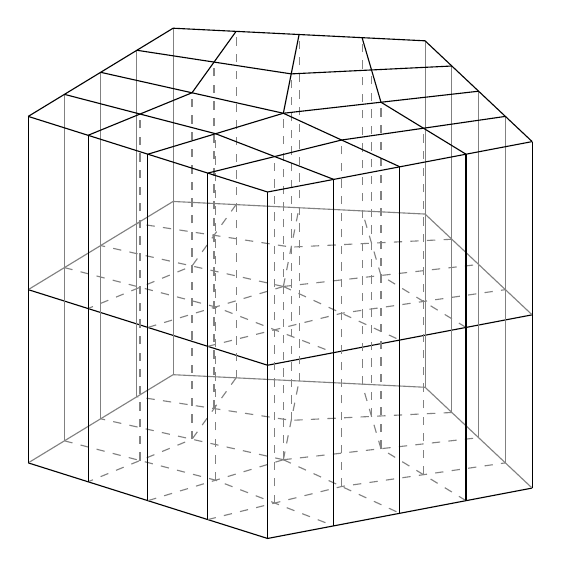
\begin{tikzpicture}[scale=0.4,%
      x={(1cm,-0.05cm)},%
      y={(0.1cm,0.5cm)},%
      z={(0cm,5.5cm)}]
      % % Bottom level
      \coordinate (root) at (0,0,0);
      \draw ($ (-8,4,0) + (root) $) -- ($ (0,0,0) + (root) $) -- ($ (8,4,0) + (root) $);
      \draw[gray] ($ (8,4,0) + (root) $) -- ($ (4,10,0) + (root) $) -- ($ (-4,10,0) + (root) $) -- ($ (-8,4,0) + (root) $);
      \draw[gray,dashed] ($ (0,5.0,0) + (root) $) -- ($ (4,2,0) + (root) $);
      \draw[gray,dashed] ($ (0,5.0,0) + (root) $) -- ($ (6,7.0,0) + (root) $);
      \draw[gray,dashed] ($ (0,5.0,0) + (root) $) -- ($ (0,10,0) + (root) $);
      \draw[gray,dashed] ($ (0,5.0,0) + (root) $) -- ($ (-6,7.0,0) + (root) $);
      \draw[gray,dashed] ($ (0,5.0,0) + (root) $) -- ($ (-4,2,0) + (root) $);
      \draw[gray,dashed] ($ (6,3.0,0) + (root) $) -- ($ (3,6,0) + (root) $) -- ($ (2,10,0) + (root) $);
      \draw[gray,dashed] ($ (5,8.5,0) + (root) $) -- ($ (0,7.5,0) + (root) $) -- ($ (-5,8.5,0) + (root) $);
      \draw[gray,dashed] ($ (-2,10,0) + (root) $) -- ($ (-3,6,0) + (root) $) -- ($ (-6,3.0,0) + (root) $);
      \draw[gray,dashed] ($ (-7,5.5,0) + (root) $) -- ($ (-2,3.5,0) + (root) $) -- ($ (2,1.0,0) + (root) $);
      \draw[gray,dashed] ($ (-2,1.0,0) + (root) $) -- ($ (2,3.5,0) + (root) $) -- ($ (7,5.5,0) + (root) $);

      % % Middle level
      \coordinate (root) at (0,0,1);
      \draw ($ (-8,4,0) + (root) $) -- ($ (0,0,0) + (root) $) -- ($ (8,4,0) + (root) $);
      \draw[gray] ($ (8,4,0) + (root) $) -- ($ (4,10,0) + (root) $) -- ($ (-4,10,0) + (root) $) -- ($ (-8,4,0) + (root) $);
      \draw[gray,dashed] ($ (0,5.0,0) + (root) $) -- ($ (4,2,0) + (root) $);
      \draw[gray,dashed] ($ (0,5.0,0) + (root) $) -- ($ (6,7.0,0) + (root) $);
      \draw[gray,dashed] ($ (0,5.0,0) + (root) $) -- ($ (0,10,0) + (root) $);
      \draw[gray,dashed] ($ (0,5.0,0) + (root) $) -- ($ (-6,7.0,0) + (root) $);
      \draw[gray,dashed] ($ (0,5.0,0) + (root) $) -- ($ (-4,2,0) + (root) $);
      \draw[gray,dashed] ($ (6,3.0,0) + (root) $) -- ($ (3,6,0) + (root) $) -- ($ (2,10,0) + (root) $);
      \draw[gray,dashed] ($ (5,8.5,0) + (root) $) -- ($ (0,7.5,0) + (root) $) -- ($ (-5,8.5,0) + (root) $);
      \draw[gray,dashed] ($ (-2,10,0) + (root) $) -- ($ (-3,6,0) + (root) $) -- ($ (-6,3.0,0) + (root) $);
      \draw[gray,dashed] ($ (-7,5.5,0) + (root) $) -- ($ (-2,3.5,0) + (root) $) -- ($ (2,1.0,0) + (root) $);
      \draw[gray,dashed] ($ (-2,1.0,0) + (root) $) -- ($ (2,3.5,0) + (root) $) -- ($ (7,5.5,0) + (root) $);

      % % Vertical lines
      \coordinate (root) at (0,0,2);
      \draw[gray] (-7,5.5,0) -- ($ (-7,5.5,0) + (root) $);
      \draw[gray,dashed] (-4.5,4.5,0) -- ($ (-4.5,4.5,0) + (root) $);
      \draw[gray,dashed] (-2,3.5,0) -- ($ (-2,3.5,0) + (root) $);
      \draw[gray,dashed] (0,2.25,0) -- ($ (0,2.25,0) + (root) $);
      \draw[gray,dashed] (2,3.5,0) -- ($ (2,3.5,0) + (root) $);
      \draw[gray,dashed] (4.5,4.5,0) -- ($ (4.5,4.5,0) + (root) $);
      \draw[gray] (7,5.5,0) -- ($ (7,5.5,0) + (root) $);
      \draw[gray] (-6,7.0,0) -- ($ (-6,7.0,0) + (root) $);
      \draw[gray,dashed] (-3,6,0) -- ($ (-3,6,0) + (root) $);
      \draw[gray,dashed] (0,5.0,0) -- ($ (0,5.0,0) + (root) $);
      \draw[gray,dashed] (3,6,0) -- ($ (3,6,0) + (root) $);
      \draw[gray] (6,7.0,0) -- ($ (6,7.0,0) + (root) $);
      \draw[gray] (-5,8.5,0) -- ($ (-5,8.5,0) + (root) $);
      \draw[gray,dashed] (-2.5,8,0) -- ($ (-2.5,8,0) + (root) $);
      \draw[gray,dashed] (0,7.5,0) -- ($ (0,7.5,0) + (root) $);
      \draw[gray,dashed] (2.5,8,0) -- ($ (2.5,8,0) + (root) $);
      \draw[gray] (5,8.5,0) -- ($ (5,8.5,0) + (root) $);
      \draw[gray] (-4,10,0) -- ($ (-4,10,0) + (root) $);
      \draw[gray,dashed] (-2,10,0) -- ($ (-2,10,0) + (root) $);
      \draw[gray,dashed] (0,10,0) -- ($ (0,10,0) + (root) $);
      \draw[gray,dashed] (2,10,0) -- ($ (2,10,0) + (root) $);
      \draw[gray] (4,10,0) -- ($ (4,10,0) + (root) $);
      \draw (-8,4,0) -- ($ (-8,4,0) + (root) $);
      \draw (-6,3.0,0) -- ($ (-6,3.0,0) + (root) $);
      \draw (-4,2,0) -- ($ (-4,2,0) + (root) $);
      \draw (-2,1.0,0) -- ($ (-2,1.0,0) + (root) $);
      \draw (0,0,0) -- ($ (0,0,0) + (root) $);
      \draw (2,1.0,0) -- ($ (2,1.0,0) + (root) $);
      \draw (4,2,0) -- ($ (4,2,0) + (root) $);
      \draw (6,3.0,0) -- ($ (6,3.0,0) + (root) $);
      \draw (8,4,0) -- ($ (8,4,0) + (root) $);

      % Top level
      \draw ($ (-8,4,0) + (root) $) -- ($ (0,0,0) + (root) $) -- ($ (8,4,0) + (root) $);
      \draw ($ (8,4,0) + (root) $) -- ($ (4,10,0) + (root) $) -- ($ (-4,10,0) + (root) $) -- ($ (-8,4,0) + (root) $);
      \draw ($ (0,5.0,0) + (root) $) -- ($ (4,2,0) + (root) $);
      \draw ($ (0,5.0,0) + (root) $) -- ($ (6,7.0,0) + (root) $);
      \draw ($ (0,5.0,0) + (root) $) -- ($ (0,10,0) + (root) $);
      \draw ($ (0,5.0,0) + (root) $) -- ($ (-6,7.0,0) + (root) $);
      \draw ($ (0,5.0,0) + (root) $) -- ($ (-4,2,0) + (root) $);
      \draw ($ (6,3.0,0) + (root) $) -- ($ (3,6,0) + (root) $) -- ($ (2,10,0) + (root) $);
      \draw ($ (5,8.5,0) + (root) $) -- ($ (0,7.5,0) + (root) $) -- ($ (-5,8.5,0) + (root) $);
      \draw ($ (-2,10,0) + (root) $) -- ($ (-3,6,0) + (root) $) -- ($ (-6,3.0,0) + (root) $);
      \draw ($ (-7,5.5,0) + (root) $) -- ($ (-2,3.5,0) + (root) $) -- ($ (2,1.0,0) + (root) $);
      \draw ($ (-2,1.0,0) + (root) $) -- ($ (2,3.5,0) + (root) $) -- ($ (7,5.5,0) + (root) $);
  \end{tikzpicture}\end{center}
\end{frame}

\begin{frame}[fragile]
  \frametitle{A more complicated example : singularities}

  \begin{center}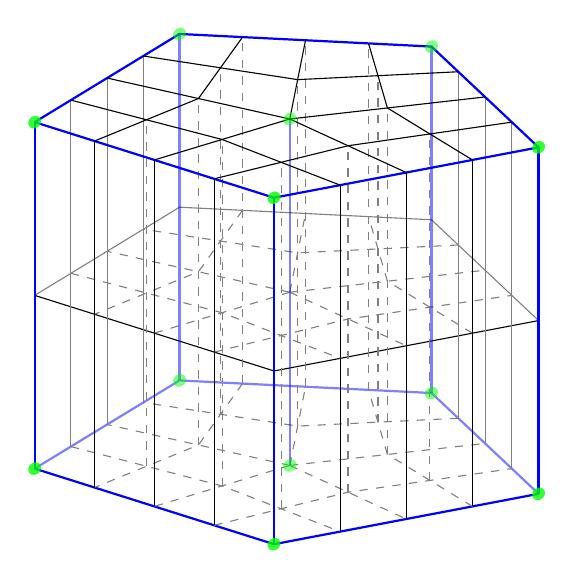
\begin{tikzpicture}[scale=0.4,%
      x={(1cm,-0.05cm)},%
      y={(0.1cm,0.5cm)},%
      z={(0cm,5.5cm)}]
      % % Bottom level
      \coordinate (root) at (0,0,0);
      \draw[thick,blue] ($ (-8,4,0) + (root) $) -- ($ (0,0,0) + (root) $) -- ($ (8,4,0) + (root) $);
      \draw[thick,blue,opacity=0.5] ($ (8,4,0) + (root) $) -- ($ (4,10,0) + (root) $) -- ($ (-4,10,0) + (root) $) -- ($ (-8,4,0) + (root) $);
      \draw[gray,dashed] ($ (0,5.0,0) + (root) $) -- ($ (4,2,0) + (root) $);
      \draw[gray,dashed] ($ (0,5.0,0) + (root) $) -- ($ (6,7.0,0) + (root) $);
      \draw[gray,dashed] ($ (0,5.0,0) + (root) $) -- ($ (0,10,0) + (root) $);
      \draw[gray,dashed] ($ (0,5.0,0) + (root) $) -- ($ (-6,7.0,0) + (root) $);
      \draw[gray,dashed] ($ (0,5.0,0) + (root) $) -- ($ (-4,2,0) + (root) $);
      \draw[gray,dashed] ($ (6,3.0,0) + (root) $) -- ($ (3,6,0) + (root) $) -- ($ (2,10,0) + (root) $);
      \draw[gray,dashed] ($ (5,8.5,0) + (root) $) -- ($ (0,7.5,0) + (root) $) -- ($ (-5,8.5,0) + (root) $);
      \draw[gray,dashed] ($ (-2,10,0) + (root) $) -- ($ (-3,6,0) + (root) $) -- ($ (-6,3.0,0) + (root) $);
      \draw[gray,dashed] ($ (-7,5.5,0) + (root) $) -- ($ (-2,3.5,0) + (root) $) -- ($ (2,1.0,0) + (root) $);
      \draw[gray,dashed] ($ (-2,1.0,0) + (root) $) -- ($ (2,3.5,0) + (root) $) -- ($ (7,5.5,0) + (root) $);

      % % Middle level
      \coordinate (root) at (0,0,1);
      \draw ($ (-8,4,0) + (root) $) -- ($ (0,0,0) + (root) $) -- ($ (8,4,0) + (root) $);
      \draw[gray] ($ (8,4,0) + (root) $) -- ($ (4,10,0) + (root) $) -- ($ (-4,10,0) + (root) $) -- ($ (-8,4,0) + (root) $);
      \draw[gray,dashed] ($ (0,5.0,0) + (root) $) -- ($ (4,2,0) + (root) $);
      \draw[gray,dashed] ($ (0,5.0,0) + (root) $) -- ($ (6,7.0,0) + (root) $);
      \draw[gray,dashed] ($ (0,5.0,0) + (root) $) -- ($ (0,10,0) + (root) $);
      \draw[gray,dashed] ($ (0,5.0,0) + (root) $) -- ($ (-6,7.0,0) + (root) $);
      \draw[gray,dashed] ($ (0,5.0,0) + (root) $) -- ($ (-4,2,0) + (root) $);
      \draw[gray,dashed] ($ (6,3.0,0) + (root) $) -- ($ (3,6,0) + (root) $) -- ($ (2,10,0) + (root) $);
      \draw[gray,dashed] ($ (5,8.5,0) + (root) $) -- ($ (0,7.5,0) + (root) $) -- ($ (-5,8.5,0) + (root) $);
      \draw[gray,dashed] ($ (-2,10,0) + (root) $) -- ($ (-3,6,0) + (root) $) -- ($ (-6,3.0,0) + (root) $);
      \draw[gray,dashed] ($ (-7,5.5,0) + (root) $) -- ($ (-2,3.5,0) + (root) $) -- ($ (2,1.0,0) + (root) $);
      \draw[gray,dashed] ($ (-2,1.0,0) + (root) $) -- ($ (2,3.5,0) + (root) $) -- ($ (7,5.5,0) + (root) $);

      % % Vertical lines
      \coordinate (root) at (0,0,2);
      \draw[gray] (-7,5.5,0) -- ($ (-7,5.5,0) + (root) $);
      \draw[gray,dashed] (-4.5,4.5,0) -- ($ (-4.5,4.5,0) + (root) $);
      \draw[gray,dashed] (-2,3.5,0) -- ($ (-2,3.5,0) + (root) $);
      \draw[gray,dashed] (0,2.25,0) -- ($ (0,2.25,0) + (root) $);
      \draw[gray,dashed] (2,3.5,0) -- ($ (2,3.5,0) + (root) $);
      \draw[gray,dashed] (4.5,4.5,0) -- ($ (4.5,4.5,0) + (root) $);
      \draw[gray] (7,5.5,0) -- ($ (7,5.5,0) + (root) $);
      \draw[gray] (-6,7.0,0) -- ($ (-6,7.0,0) + (root) $);
      \draw[gray,dashed] (-3,6,0) -- ($ (-3,6,0) + (root) $);
      \draw[thick,blue,opacity=0.5] (0,5.0,0) -- ($ (0,5.0,0) + (root) $);
      \draw[gray,dashed] (3,6,0) -- ($ (3,6,0) + (root) $);
      \draw[gray] (6,7.0,0) -- ($ (6,7.0,0) + (root) $);
      \draw[gray] (-5,8.5,0) -- ($ (-5,8.5,0) + (root) $);
      \draw[gray,dashed] (-2.5,8,0) -- ($ (-2.5,8,0) + (root) $);
      \draw[gray,dashed] (0,7.5,0) -- ($ (0,7.5,0) + (root) $);
      \draw[gray,dashed] (2.5,8,0) -- ($ (2.5,8,0) + (root) $);
      \draw[gray] (5,8.5,0) -- ($ (5,8.5,0) + (root) $);
      \draw[thick,blue,opacity=0.5] (-4,10,0) -- ($ (-4,10,0) + (root) $);
      \draw[gray,dashed] (-2,10,0) -- ($ (-2,10,0) + (root) $);
      \draw[gray,dashed] (0,10,0) -- ($ (0,10,0) + (root) $);
      \draw[gray,dashed] (2,10,0) -- ($ (2,10,0) + (root) $);
      \draw[thick,blue,opacity=0.5] (4,10,0) -- ($ (4,10,0) + (root) $);
      \draw[thick,blue] (-8,4,0) -- ($ (-8,4,0) + (root) $);
      \draw (-6,3.0,0) -- ($ (-6,3.0,0) + (root) $);
      \draw (-4,2,0) -- ($ (-4,2,0) + (root) $);
      \draw (-2,1.0,0) -- ($ (-2,1.0,0) + (root) $);
      \draw[thick,blue] (0,0,0) -- ($ (0,0,0) + (root) $);
      \draw (2,1.0,0) -- ($ (2,1.0,0) + (root) $);
      \draw (4,2,0) -- ($ (4,2,0) + (root) $);
      \draw (6,3.0,0) -- ($ (6,3.0,0) + (root) $);
      \draw[thick,blue] (8,4,0) -- ($ (8,4,0) + (root) $);

      % Top level
      \draw[thick,blue] ($ (-8,4,0) + (root) $) -- ($ (0,0,0) + (root) $) -- ($ (8,4,0) + (root) $);
      \draw[thick,blue] ($ (8,4,0) + (root) $) -- ($ (4,10,0) + (root) $) -- ($ (-4,10,0) + (root) $) -- ($ (-8,4,0) + (root) $);
      \draw ($ (0,5.0,0) + (root) $) -- ($ (4,2,0) + (root) $);
      \draw ($ (0,5.0,0) + (root) $) -- ($ (6,7.0,0) + (root) $);
      \draw ($ (0,5.0,0) + (root) $) -- ($ (0,10,0) + (root) $);
      \draw ($ (0,5.0,0) + (root) $) -- ($ (-6,7.0,0) + (root) $);
      \draw ($ (0,5.0,0) + (root) $) -- ($ (-4,2,0) + (root) $);
      \draw ($ (6,3.0,0) + (root) $) -- ($ (3,6,0) + (root) $) -- ($ (2,10,0) + (root) $);
      \draw ($ (5,8.5,0) + (root) $) -- ($ (0,7.5,0) + (root) $) -- ($ (-5,8.5,0) + (root) $);
      \draw ($ (-2,10,0) + (root) $) -- ($ (-3,6,0) + (root) $) -- ($ (-6,3.0,0) + (root) $);
      \draw ($ (-7,5.5,0) + (root) $) -- ($ (-2,3.5,0) + (root) $) -- ($ (2,1.0,0) + (root) $);
      \draw ($ (-2,1.0,0) + (root) $) -- ($ (2,3.5,0) + (root) $) -- ($ (7,5.5,0) + (root) $);

      % Singular vertices
      \fill[color=green,fill=green,opacity=0.8] (0,0,0) ellipse (0.2 and 0.4);
      \fill[color=green,fill=green,opacity=0.8] (-8,4,0) ellipse (0.2 and 0.4);
      \fill[color=green,fill=green,opacity=0.8] (8,4,0) ellipse (0.2 and 0.4);
      \fill[color=green,fill=green,opacity=0.5] (0,5,0) ellipse (0.2 and 0.4);
      \fill[color=green,fill=green,opacity=0.5] (-4,10,0) ellipse (0.2 and 0.4);
      \fill[color=green,fill=green,opacity=0.5] (4,10,0) ellipse (0.2 and 0.4);
      \fill[color=green,fill=green,opacity=0.8] (0,0,2) ellipse (0.2 and 0.4);
      \fill[color=green,fill=green,opacity=0.8] (-8,4,2) ellipse (0.2 and 0.4);
      \fill[color=green,fill=green,opacity=0.8] (8,4,2) ellipse (0.2 and 0.4);
      \fill[color=green,fill=green,opacity=0.5] (0,5,2) ellipse (0.2 and 0.4);
      \fill[color=green,fill=green,opacity=0.5] (-4,10,2) ellipse (0.2 and 0.4);
      \fill[color=green,fill=green,opacity=0.5] (4,10,2) ellipse (0.2 and 0.4);
  \end{tikzpicture}\end{center}
\end{frame}

\begin{frame}[fragile]
  \frametitle{Separation surface}

  \begin{center}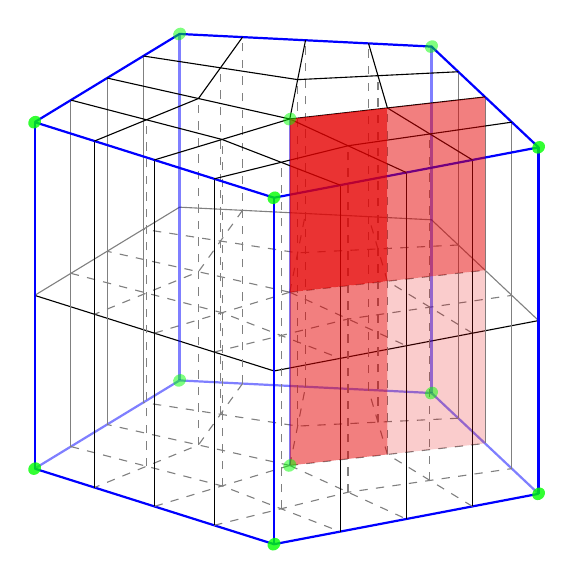
\begin{tikzpicture}[scale=0.4,%
      x={(1cm,-0.05cm)},%
      y={(0.1cm,0.5cm)},%
      z={(0cm,5.5cm)}]
      % % Bottom level
      \coordinate (root) at (0,0,0);
      \draw[thick,blue] ($ (-8,4,0) + (root) $) -- ($ (0,0,0) + (root) $) -- ($ (8,4,0) + (root) $);
      \draw[thick,blue,opacity=0.5] ($ (8,4,0) + (root) $) -- ($ (4,10,0) + (root) $) -- ($ (-4,10,0) + (root) $) -- ($ (-8,4,0) + (root) $);
      \draw[gray,dashed] ($ (0,5.0,0) + (root) $) -- ($ (4,2,0) + (root) $);
      \draw[gray,dashed] ($ (0,5.0,0) + (root) $) -- ($ (6,7.0,0) + (root) $);
      \draw[gray,dashed] ($ (0,5.0,0) + (root) $) -- ($ (0,10,0) + (root) $);
      \draw[gray,dashed] ($ (0,5.0,0) + (root) $) -- ($ (-6,7.0,0) + (root) $);
      \draw[gray,dashed] ($ (0,5.0,0) + (root) $) -- ($ (-4,2,0) + (root) $);
      \draw[gray,dashed] ($ (6,3.0,0) + (root) $) -- ($ (3,6,0) + (root) $) -- ($ (2,10,0) + (root) $);
      \draw[gray,dashed] ($ (5,8.5,0) + (root) $) -- ($ (0,7.5,0) + (root) $) -- ($ (-5,8.5,0) + (root) $);
      \draw[gray,dashed] ($ (-2,10,0) + (root) $) -- ($ (-3,6,0) + (root) $) -- ($ (-6,3.0,0) + (root) $);
      \draw[gray,dashed] ($ (-7,5.5,0) + (root) $) -- ($ (-2,3.5,0) + (root) $) -- ($ (2,1.0,0) + (root) $);
      \draw[gray,dashed] ($ (-2,1.0,0) + (root) $) -- ($ (2,3.5,0) + (root) $) -- ($ (7,5.5,0) + (root) $);

      % % Middle level
      \coordinate (root) at (0,0,1);
      \draw ($ (-8,4,0) + (root) $) -- ($ (0,0,0) + (root) $) -- ($ (8,4,0) + (root) $);
      \draw[gray] ($ (8,4,0) + (root) $) -- ($ (4,10,0) + (root) $) -- ($ (-4,10,0) + (root) $) -- ($ (-8,4,0) + (root) $);
      \draw[gray,dashed] ($ (0,5.0,0) + (root) $) -- ($ (4,2,0) + (root) $);
      \draw[gray,dashed] ($ (0,5.0,0) + (root) $) -- ($ (6,7.0,0) + (root) $);
      \draw[gray,dashed] ($ (0,5.0,0) + (root) $) -- ($ (0,10,0) + (root) $);
      \draw[gray,dashed] ($ (0,5.0,0) + (root) $) -- ($ (-6,7.0,0) + (root) $);
      \draw[gray,dashed] ($ (0,5.0,0) + (root) $) -- ($ (-4,2,0) + (root) $);
      \draw[gray,dashed] ($ (6,3.0,0) + (root) $) -- ($ (3,6,0) + (root) $) -- ($ (2,10,0) + (root) $);
      \draw[gray,dashed] ($ (5,8.5,0) + (root) $) -- ($ (0,7.5,0) + (root) $) -- ($ (-5,8.5,0) + (root) $);
      \draw[gray,dashed] ($ (-2,10,0) + (root) $) -- ($ (-3,6,0) + (root) $) -- ($ (-6,3.0,0) + (root) $);
      \draw[gray,dashed] ($ (-7,5.5,0) + (root) $) -- ($ (-2,3.5,0) + (root) $) -- ($ (2,1.0,0) + (root) $);
      \draw[gray,dashed] ($ (-2,1.0,0) + (root) $) -- ($ (2,3.5,0) + (root) $) -- ($ (7,5.5,0) + (root) $);

      % % Vertical lines
      \coordinate (root) at (0,0,2);
      \draw[gray] (-7,5.5,0) -- ($ (-7,5.5,0) + (root) $);
      \draw[gray,dashed] (-4.5,4.5,0) -- ($ (-4.5,4.5,0) + (root) $);
      \draw[gray,dashed] (-2,3.5,0) -- ($ (-2,3.5,0) + (root) $);
      \draw[gray,dashed] (0,2.25,0) -- ($ (0,2.25,0) + (root) $);
      \draw[gray,dashed] (2,3.5,0) -- ($ (2,3.5,0) + (root) $);
      \draw[gray,dashed] (4.5,4.5,0) -- ($ (4.5,4.5,0) + (root) $);
      \draw[gray] (7,5.5,0) -- ($ (7,5.5,0) + (root) $);
      \draw[gray] (-6,7.0,0) -- ($ (-6,7.0,0) + (root) $);
      \draw[gray,dashed] (-3,6,0) -- ($ (-3,6,0) + (root) $);
      \draw[thick,blue,opacity=0.5] (0,5.0,0) -- ($ (0,5.0,0) + (root) $);
      \draw[gray,dashed] (3,6,0) -- ($ (3,6,0) + (root) $);
      \draw[gray] (6,7.0,0) -- ($ (6,7.0,0) + (root) $);
      \draw[gray] (-5,8.5,0) -- ($ (-5,8.5,0) + (root) $);
      \draw[gray,dashed] (-2.5,8,0) -- ($ (-2.5,8,0) + (root) $);
      \draw[gray,dashed] (0,7.5,0) -- ($ (0,7.5,0) + (root) $);
      \draw[gray,dashed] (2.5,8,0) -- ($ (2.5,8,0) + (root) $);
      \draw[gray] (5,8.5,0) -- ($ (5,8.5,0) + (root) $);
      \draw[thick,blue,opacity=0.5] (-4,10,0) -- ($ (-4,10,0) + (root) $);
      \draw[gray,dashed] (-2,10,0) -- ($ (-2,10,0) + (root) $);
      \draw[gray,dashed] (0,10,0) -- ($ (0,10,0) + (root) $);
      \draw[gray,dashed] (2,10,0) -- ($ (2,10,0) + (root) $);
      \draw[thick,blue,opacity=0.5] (4,10,0) -- ($ (4,10,0) + (root) $);
      \draw[thick,blue] (-8,4,0) -- ($ (-8,4,0) + (root) $);
      \draw (-6,3.0,0) -- ($ (-6,3.0,0) + (root) $);
      \draw (-4,2,0) -- ($ (-4,2,0) + (root) $);
      \draw (-2,1.0,0) -- ($ (-2,1.0,0) + (root) $);
      \draw[thick,blue] (0,0,0) -- ($ (0,0,0) + (root) $);
      \draw (2,1.0,0) -- ($ (2,1.0,0) + (root) $);
      \draw (4,2,0) -- ($ (4,2,0) + (root) $);
      \draw (6,3.0,0) -- ($ (6,3.0,0) + (root) $);
      \draw[thick,blue] (8,4,0) -- ($ (8,4,0) + (root) $);

      % Top level
      \draw[thick,blue] ($ (-8,4,0) + (root) $) -- ($ (0,0,0) + (root) $) -- ($ (8,4,0) + (root) $);
      \draw[thick,blue] ($ (8,4,0) + (root) $) -- ($ (4,10,0) + (root) $) -- ($ (-4,10,0) + (root) $) -- ($ (-8,4,0) + (root) $);
      \draw ($ (0,5.0,0) + (root) $) -- ($ (4,2,0) + (root) $);
      \draw ($ (0,5.0,0) + (root) $) -- ($ (6,7.0,0) + (root) $);
      \draw ($ (0,5.0,0) + (root) $) -- ($ (0,10,0) + (root) $);
      \draw ($ (0,5.0,0) + (root) $) -- ($ (-6,7.0,0) + (root) $);
      \draw ($ (0,5.0,0) + (root) $) -- ($ (-4,2,0) + (root) $);
      \draw ($ (6,3.0,0) + (root) $) -- ($ (3,6,0) + (root) $) -- ($ (2,10,0) + (root) $);
      \draw ($ (5,8.5,0) + (root) $) -- ($ (0,7.5,0) + (root) $) -- ($ (-5,8.5,0) + (root) $);
      \draw ($ (-2,10,0) + (root) $) -- ($ (-3,6,0) + (root) $) -- ($ (-6,3.0,0) + (root) $);
      \draw ($ (-7,5.5,0) + (root) $) -- ($ (-2,3.5,0) + (root) $) -- ($ (2,1.0,0) + (root) $);
      \draw ($ (-2,1.0,0) + (root) $) -- ($ (2,3.5,0) + (root) $) -- ($ (7,5.5,0) + (root) $);

      % Separation surface 1
      \fill[color=red,fill=red,opacity=0.8] (0,5,1) -- (3,6,1) -- (3,6,2) -- (0,5,2) -- cycle;
      \fill[color=red,fill=red,opacity=0.5] (3,6,1) -- (6,7,1) -- (6,7,2) -- (3,6,2) -- cycle;
      \fill[color=red,fill=red,opacity=0.5] (0,5,1) -- (3,6,1) -- (3,6,0) -- (0,5,0) -- cycle;
      \fill[color=red,fill=red,opacity=0.2] (3,6,1) -- (6,7,1) -- (6,7,0) -- (3,6,0) -- cycle;

      % Singular vertices
      \fill[color=green,fill=green,opacity=0.8] (0,0,0) ellipse (0.2 and 0.4);
      \fill[color=green,fill=green,opacity=0.8] (-8,4,0) ellipse (0.2 and 0.4);
      \fill[color=green,fill=green,opacity=0.8] (8,4,0) ellipse (0.2 and 0.4);
      \fill[color=green,fill=green,opacity=0.5] (0,5,0) ellipse (0.2 and 0.4);
      \fill[color=green,fill=green,opacity=0.5] (-4,10,0) ellipse (0.2 and 0.4);
      \fill[color=green,fill=green,opacity=0.5] (4,10,0) ellipse (0.2 and 0.4);
      \fill[color=green,fill=green,opacity=0.8] (0,0,2) ellipse (0.2 and 0.4);
      \fill[color=green,fill=green,opacity=0.8] (-8,4,2) ellipse (0.2 and 0.4);
      \fill[color=green,fill=green,opacity=0.8] (8,4,2) ellipse (0.2 and 0.4);
      \fill[color=green,fill=green,opacity=0.5] (0,5,2) ellipse (0.2 and 0.4);
      \fill[color=green,fill=green,opacity=0.5] (-4,10,2) ellipse (0.2 and 0.4);
      \fill[color=green,fill=green,opacity=0.5] (4,10,2) ellipse (0.2 and 0.4);
  \end{tikzpicture}\end{center}
\end{frame}

\begin{frame}[fragile]
  \frametitle{Base complex}

  \begin{center}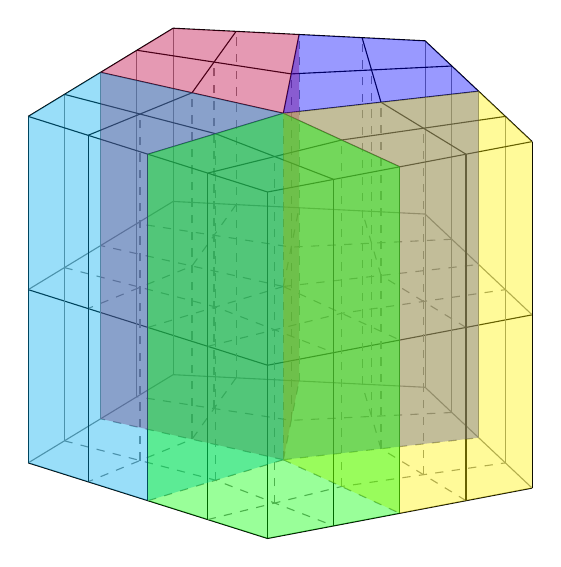
\begin{tikzpicture}[scale=0.4,%
      x={(1cm,-0.05cm)},%
      y={(0.1cm,0.5cm)},%
      z={(0cm,5.5cm)}]
      % % Bottom level
      \coordinate (root) at (0,0,0);
      \draw ($ (-8,4,0) + (root) $) -- ($ (0,0,0) + (root) $) -- ($ (8,4,0) + (root) $);
      \draw[gray] ($ (8,4,0) + (root) $) -- ($ (4,10,0) + (root) $) -- ($ (-4,10,0) + (root) $) -- ($ (-8,4,0) + (root) $);
      \draw[gray,dashed] ($ (0,5.0,0) + (root) $) -- ($ (4,2,0) + (root) $);
      \draw[gray,dashed] ($ (0,5.0,0) + (root) $) -- ($ (6,7.0,0) + (root) $);
      \draw[gray,dashed] ($ (0,5.0,0) + (root) $) -- ($ (0,10,0) + (root) $);
      \draw[gray,dashed] ($ (0,5.0,0) + (root) $) -- ($ (-6,7.0,0) + (root) $);
      \draw[gray,dashed] ($ (0,5.0,0) + (root) $) -- ($ (-4,2,0) + (root) $);
      \draw[gray,dashed] ($ (6,3.0,0) + (root) $) -- ($ (3,6,0) + (root) $) -- ($ (2,10,0) + (root) $);
      \draw[gray,dashed] ($ (5,8.5,0) + (root) $) -- ($ (0,7.5,0) + (root) $) -- ($ (-5,8.5,0) + (root) $);
      \draw[gray,dashed] ($ (-2,10,0) + (root) $) -- ($ (-3,6,0) + (root) $) -- ($ (-6,3.0,0) + (root) $);
      \draw[gray,dashed] ($ (-7,5.5,0) + (root) $) -- ($ (-2,3.5,0) + (root) $) -- ($ (2,1.0,0) + (root) $);
      \draw[gray,dashed] ($ (-2,1.0,0) + (root) $) -- ($ (2,3.5,0) + (root) $) -- ($ (7,5.5,0) + (root) $);

      % % Middle level
      \coordinate (root) at (0,0,1);
      \draw ($ (-8,4,0) + (root) $) -- ($ (0,0,0) + (root) $) -- ($ (8,4,0) + (root) $);
      \draw[gray] ($ (8,4,0) + (root) $) -- ($ (4,10,0) + (root) $) -- ($ (-4,10,0) + (root) $) -- ($ (-8,4,0) + (root) $);
      \draw[gray,dashed] ($ (0,5.0,0) + (root) $) -- ($ (4,2,0) + (root) $);
      \draw[gray,dashed] ($ (0,5.0,0) + (root) $) -- ($ (6,7.0,0) + (root) $);
      \draw[gray,dashed] ($ (0,5.0,0) + (root) $) -- ($ (0,10,0) + (root) $);
      \draw[gray,dashed] ($ (0,5.0,0) + (root) $) -- ($ (-6,7.0,0) + (root) $);
      \draw[gray,dashed] ($ (0,5.0,0) + (root) $) -- ($ (-4,2,0) + (root) $);
      \draw[gray,dashed] ($ (6,3.0,0) + (root) $) -- ($ (3,6,0) + (root) $) -- ($ (2,10,0) + (root) $);
      \draw[gray,dashed] ($ (5,8.5,0) + (root) $) -- ($ (0,7.5,0) + (root) $) -- ($ (-5,8.5,0) + (root) $);
      \draw[gray,dashed] ($ (-2,10,0) + (root) $) -- ($ (-3,6,0) + (root) $) -- ($ (-6,3.0,0) + (root) $);
      \draw[gray,dashed] ($ (-7,5.5,0) + (root) $) -- ($ (-2,3.5,0) + (root) $) -- ($ (2,1.0,0) + (root) $);
      \draw[gray,dashed] ($ (-2,1.0,0) + (root) $) -- ($ (2,3.5,0) + (root) $) -- ($ (7,5.5,0) + (root) $);

      % % Vertical lines
      \coordinate (root) at (0,0,2);
      \draw[gray] (-7,5.5,0) -- ($ (-7,5.5,0) + (root) $);
      \draw[gray,dashed] (-4.5,4.5,0) -- ($ (-4.5,4.5,0) + (root) $);
      \draw[gray,dashed] (-2,3.5,0) -- ($ (-2,3.5,0) + (root) $);
      \draw[gray,dashed] (0,2.25,0) -- ($ (0,2.25,0) + (root) $);
      \draw[gray,dashed] (2,3.5,0) -- ($ (2,3.5,0) + (root) $);
      \draw[gray,dashed] (4.5,4.5,0) -- ($ (4.5,4.5,0) + (root) $);
      \draw[gray] (7,5.5,0) -- ($ (7,5.5,0) + (root) $);
      \draw[gray] (-6,7.0,0) -- ($ (-6,7.0,0) + (root) $);
      \draw[gray,dashed] (-3,6,0) -- ($ (-3,6,0) + (root) $);
      \draw[gray,dashed] (0,5.0,0) -- ($ (0,5.0,0) + (root) $);
      \draw[gray,dashed] (3,6,0) -- ($ (3,6,0) + (root) $);
      \draw[gray] (6,7.0,0) -- ($ (6,7.0,0) + (root) $);
      \draw[gray] (-5,8.5,0) -- ($ (-5,8.5,0) + (root) $);
      \draw[gray,dashed] (-2.5,8,0) -- ($ (-2.5,8,0) + (root) $);
      \draw[gray,dashed] (0,7.5,0) -- ($ (0,7.5,0) + (root) $);
      \draw[gray,dashed] (2.5,8,0) -- ($ (2.5,8,0) + (root) $);
      \draw[gray] (5,8.5,0) -- ($ (5,8.5,0) + (root) $);
      \draw[gray] (-4,10,0) -- ($ (-4,10,0) + (root) $);
      \draw[gray,dashed] (-2,10,0) -- ($ (-2,10,0) + (root) $);
      \draw[gray,dashed] (0,10,0) -- ($ (0,10,0) + (root) $);
      \draw[gray,dashed] (2,10,0) -- ($ (2,10,0) + (root) $);
      \draw[gray] (4,10,0) -- ($ (4,10,0) + (root) $);
      \draw (-8,4,0) -- ($ (-8,4,0) + (root) $);
      \draw (-6,3.0,0) -- ($ (-6,3.0,0) + (root) $);
      \draw (-4,2,0) -- ($ (-4,2,0) + (root) $);
      \draw (-2,1.0,0) -- ($ (-2,1.0,0) + (root) $);
      \draw (0,0,0) -- ($ (0,0,0) + (root) $);
      \draw (2,1.0,0) -- ($ (2,1.0,0) + (root) $);
      \draw (4,2,0) -- ($ (4,2,0) + (root) $);
      \draw (6,3.0,0) -- ($ (6,3.0,0) + (root) $);
      \draw (8,4,0) -- ($ (8,4,0) + (root) $);

      % Top level
      \draw ($ (-8,4,0) + (root) $) -- ($ (0,0,0) + (root) $) -- ($ (8,4,0) + (root) $);
      \draw ($ (8,4,0) + (root) $) -- ($ (4,10,0) + (root) $) -- ($ (-4,10,0) + (root) $) -- ($ (-8,4,0) + (root) $);
      \draw ($ (0,5.0,0) + (root) $) -- ($ (4,2,0) + (root) $);
      \draw ($ (0,5.0,0) + (root) $) -- ($ (6,7.0,0) + (root) $);
      \draw ($ (0,5.0,0) + (root) $) -- ($ (0,10,0) + (root) $);
      \draw ($ (0,5.0,0) + (root) $) -- ($ (-6,7.0,0) + (root) $);
      \draw ($ (0,5.0,0) + (root) $) -- ($ (-4,2,0) + (root) $);
      \draw ($ (6,3.0,0) + (root) $) -- ($ (3,6,0) + (root) $) -- ($ (2,10,0) + (root) $);
      \draw ($ (5,8.5,0) + (root) $) -- ($ (0,7.5,0) + (root) $) -- ($ (-5,8.5,0) + (root) $);
      \draw ($ (-2,10,0) + (root) $) -- ($ (-3,6,0) + (root) $) -- ($ (-6,3.0,0) + (root) $);
      \draw ($ (-7,5.5,0) + (root) $) -- ($ (-2,3.5,0) + (root) $) -- ($ (2,1.0,0) + (root) $);
      \draw ($ (-2,1.0,0) + (root) $) -- ($ (2,3.5,0) + (root) $) -- ($ (7,5.5,0) + (root) $);

      % Components
      \fill[color=red,fill=purple,opacity=0.4] (-4,10,2) -- (-6,7,2) -- (-6,7,0) -- (0,5,0) -- (0,10,0) -- (0,10,2) -- cycle;
      \fill[color=blue,fill=blue,opacity=0.4] (0,10,2) -- (4,10,2) -- (6,7,2) -- (6,7,0) -- (0,5,0) -- (0,5,2) -- cycle;
      \fill[color=cyan,fill=cyan,opacity=0.4] (-6,7,2) -- (0,5,2) -- (0,5,0) -- (-4,2,0) -- (-8,4,0) -- (-8,4,2) -- cycle;
      \fill[color=yellow,fill=yellow,opacity=0.4] (6,7,2) -- (0,5,2) -- (0,5,0) -- (4,2,0) -- (8,4,0) -- (8,4,2) -- cycle;
      \fill[color=green,fill=green,opacity=0.4] (0,0,0) -- (4,2,0) -- (4,2,2) -- (0,5,2) -- (-4,2,2) -- (-4,2,0) -- cycle;
  \end{tikzpicture}\end{center}
\end{frame}

\begin{frame}
  \frametitle{Circular base component}

  \begin{center}
    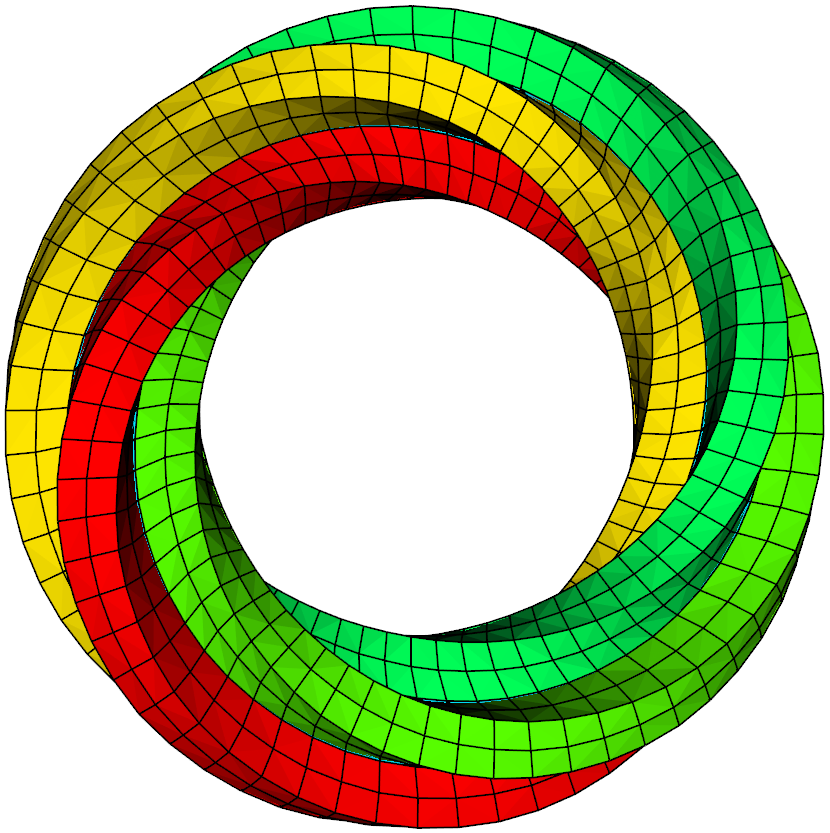
\includegraphics[height=0.8\textheight]{./images/circular-base.png}
  \end{center}
\end{frame}

\begin{frame}[fragile]
  \frametitle{Real example 1}
  \begin{columns}
    \begin{column}{0.5\textwidth}
      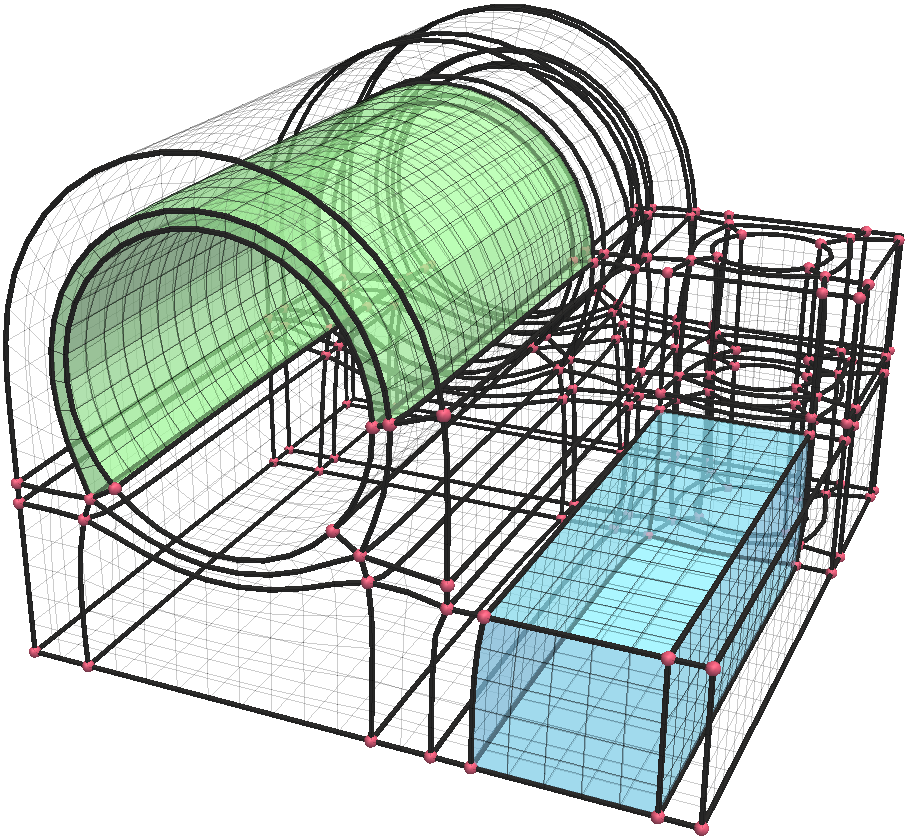
\includegraphics[width=\textwidth]{./images/ex1-singularities.png}
    \end{column}
    \begin{column}{0.5\textwidth}
      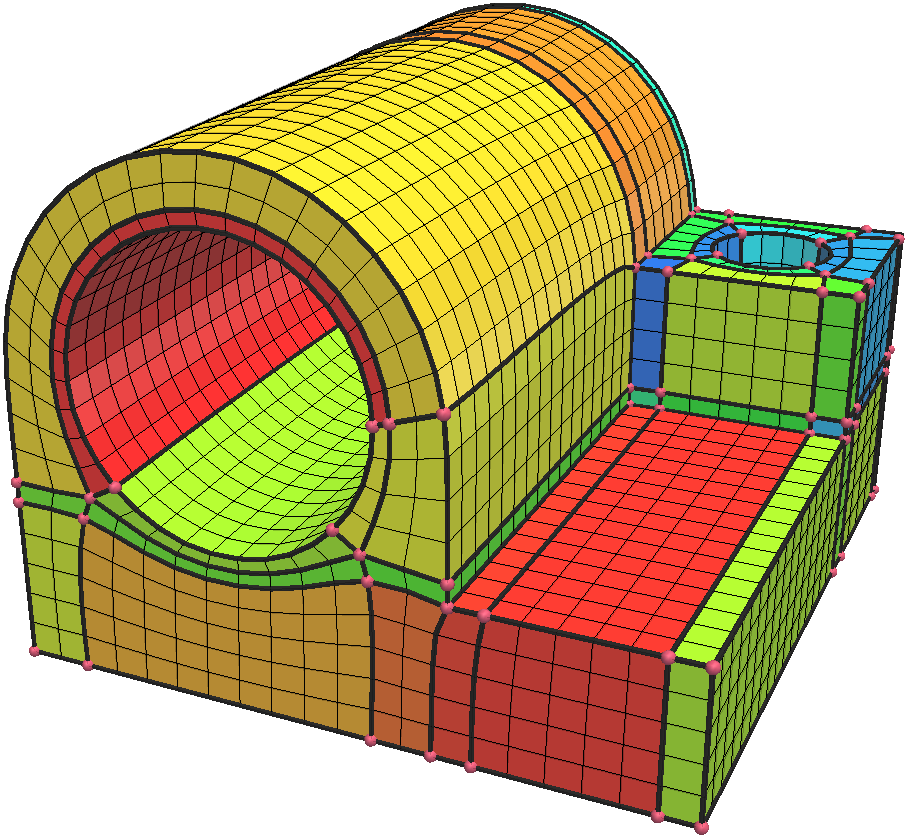
\includegraphics[width=\textwidth]{./images/ex1-base-complex.png}
    \end{column}
  \end{columns}
\end{frame}

\begin{frame}[fragile]
  \frametitle{Real example 2}
  \begin{columns}
    \begin{column}{0.5\textwidth}
      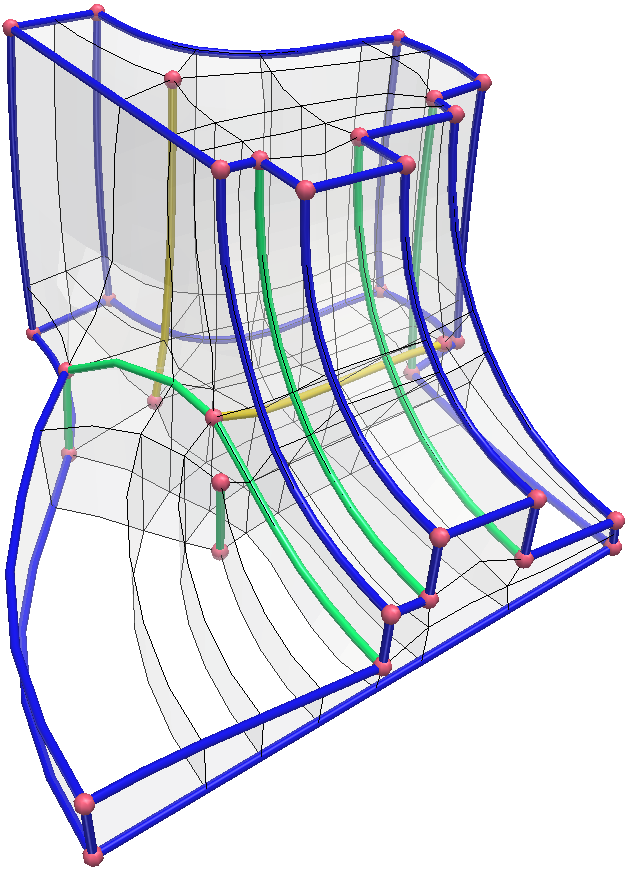
\includegraphics[width=\textwidth]{./images/ex2-singularities.png}
    \end{column}
    \begin{column}{0.5\textwidth}
      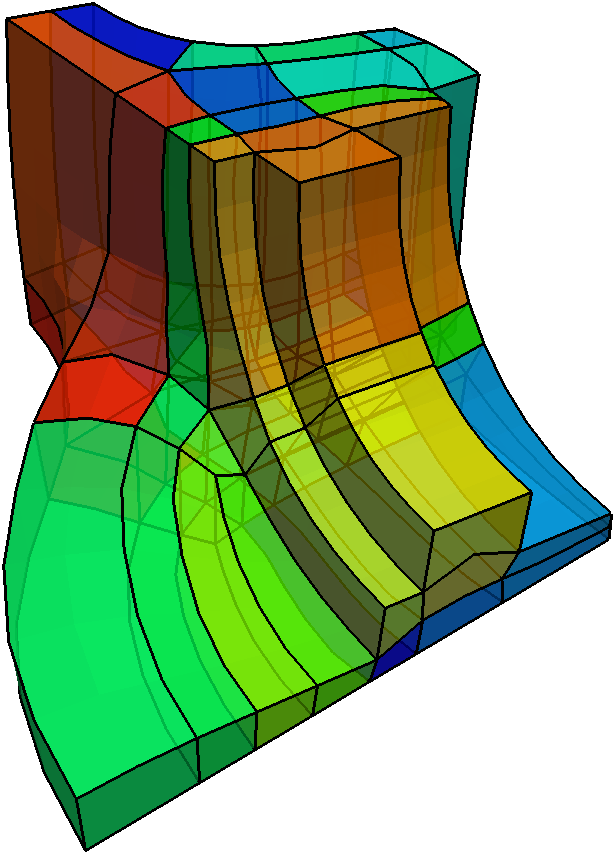
\includegraphics[width=\textwidth]{./images/ex2-base-complex.png}
    \end{column}
  \end{columns}
\end{frame}

\begin{frame}[fragile]
  \frametitle{Sheets}
  \begin{center}
    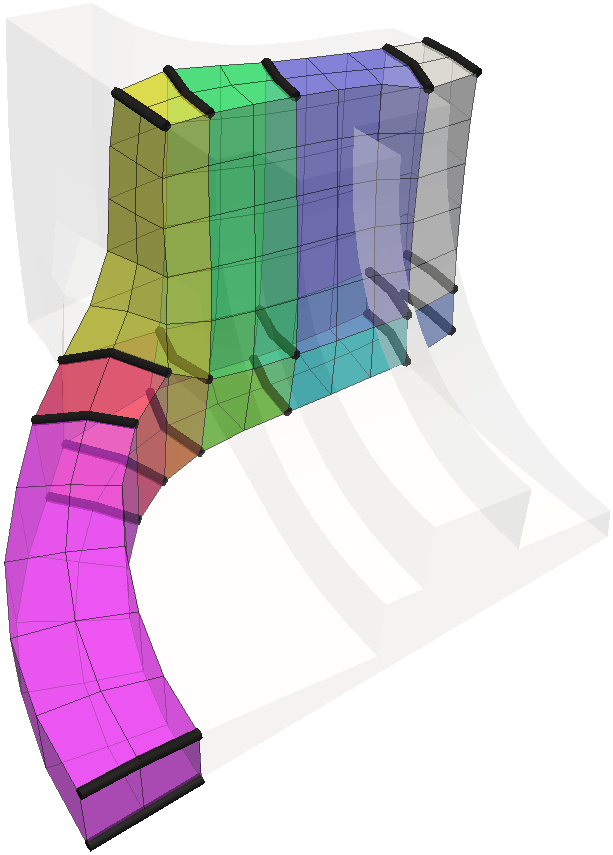
\includegraphics[height=0.8\textheight]{./images/ex2-sheet1.png}
  \end{center}
\end{frame}

\section{Visualisation}

% TODO

\section{Selection}

\begin{frame}
  \frametitle{Sheet complexity}
  \begin{center}
    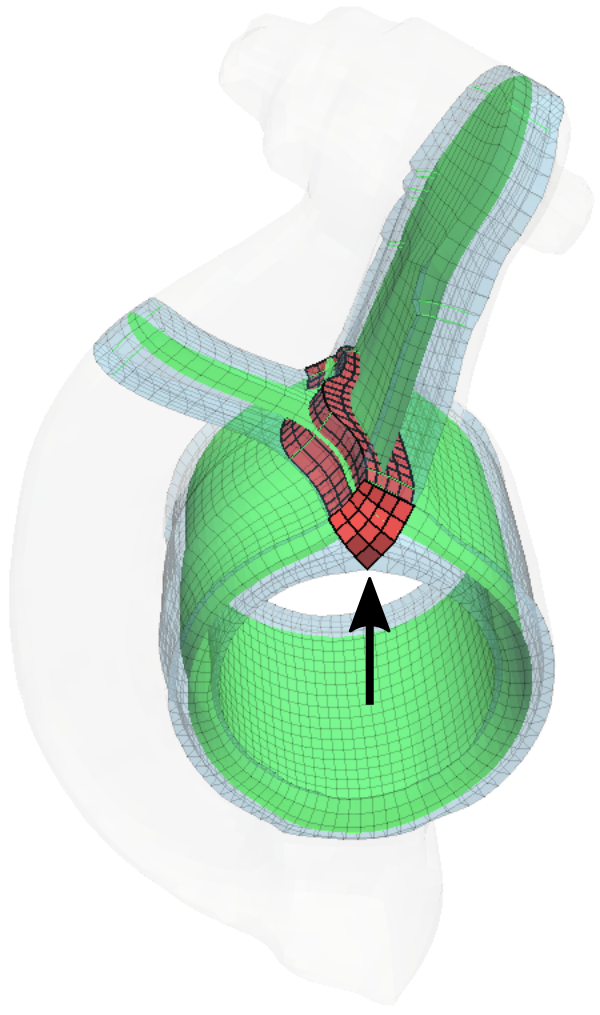
\includegraphics[height=0.8\textheight]{./images/self-intersect.png}
  \end{center}
\end{frame}

\begin{frame}
  \frametitle{Sheets interactions}
  \begin{columns}
    \begin{column}{0.3\textwidth}
      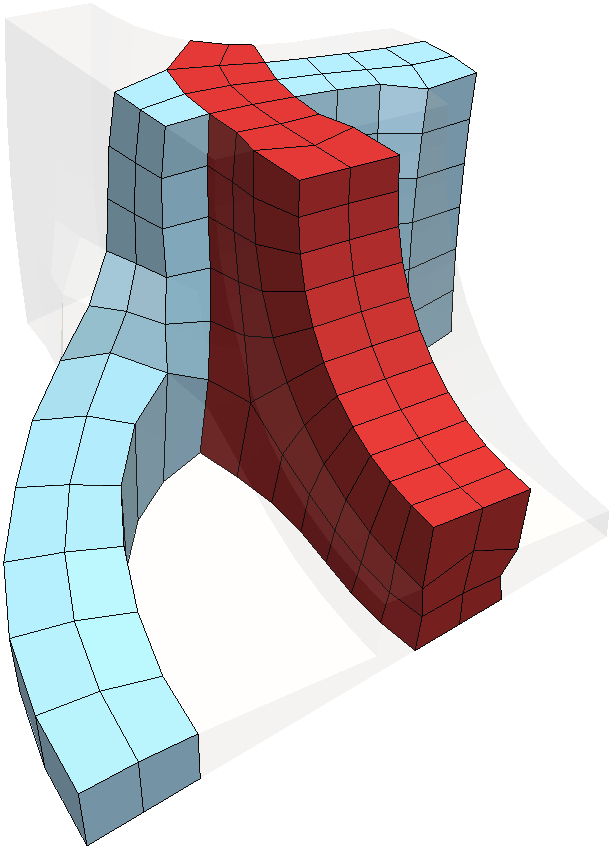
\includegraphics[width=\textwidth]{./images/sheet-intersect.png}
      \begin{center}Intersecting\end{center}
    \end{column}
    \begin{column}{0.3\textwidth}
      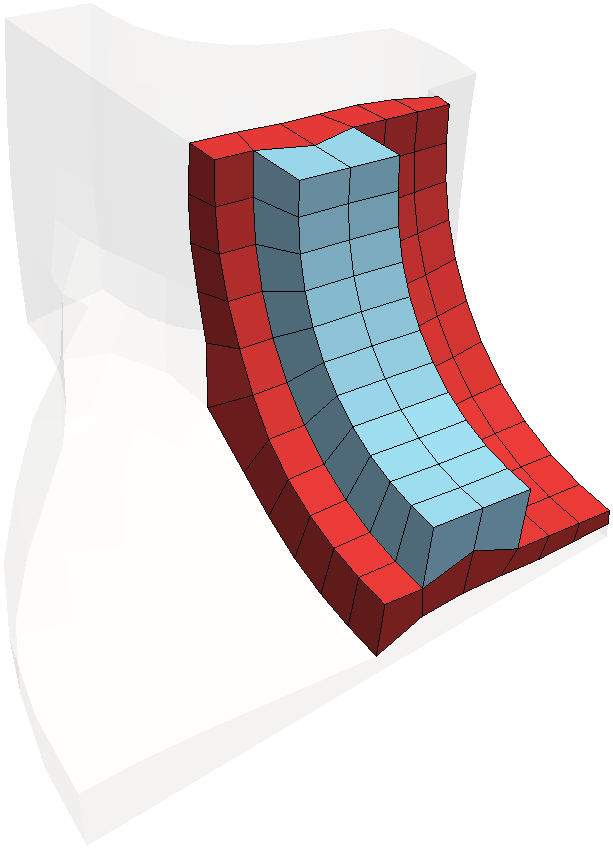
\includegraphics[width=\textwidth]{./images/sheet-adjacent.png}
      \begin{center}Adjacent\end{center}
    \end{column}
    \begin{column}{0.3\textwidth}
      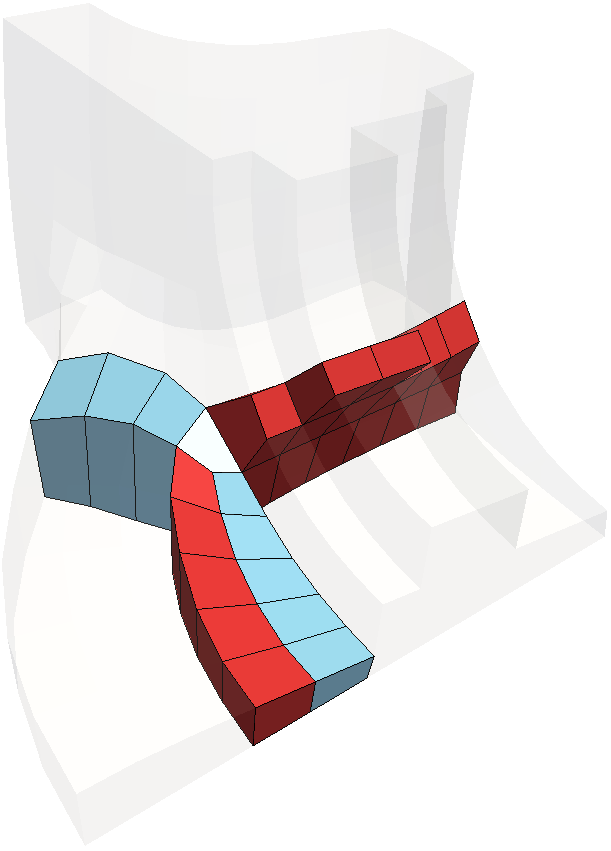
\includegraphics[width=\textwidth]{./images/sheet-hybrid.png}
      \begin{center}Hybrid\end{center}
    \end{column}
  \end{columns}
\end{frame}

\begin{frame}
  \frametitle{Sheet covering selection}

  \begin{itemize}
    \item Cover all base complexes
    \item Minimize the intersection of sheets
    \item Maximize individual sheet complexity
  \end{itemize}

  \begin{block}{Remark}
    This is a special case of the set cover problem.
  \end{block}
\end{frame}

\begin{frame}
  \frametitle{Sheet interaction matrix}
  \begin{columns}
    \begin{column}{0.5\textwidth}
      \begin{center}
        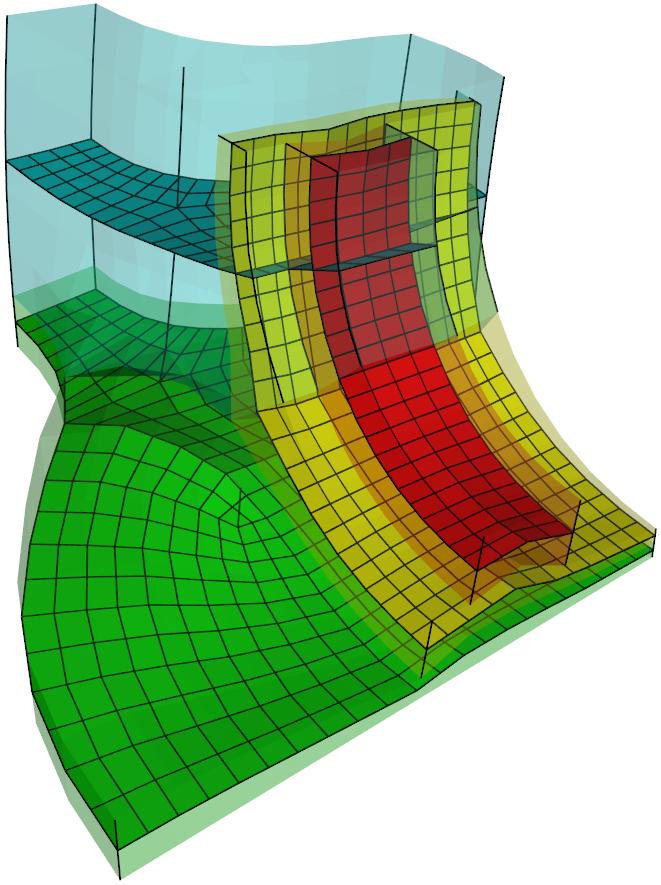
\includegraphics[height=\textwidth]{./images/interaction.png}
      \end{center}
    \end{column}
    \begin{column}{0.5\textwidth}
      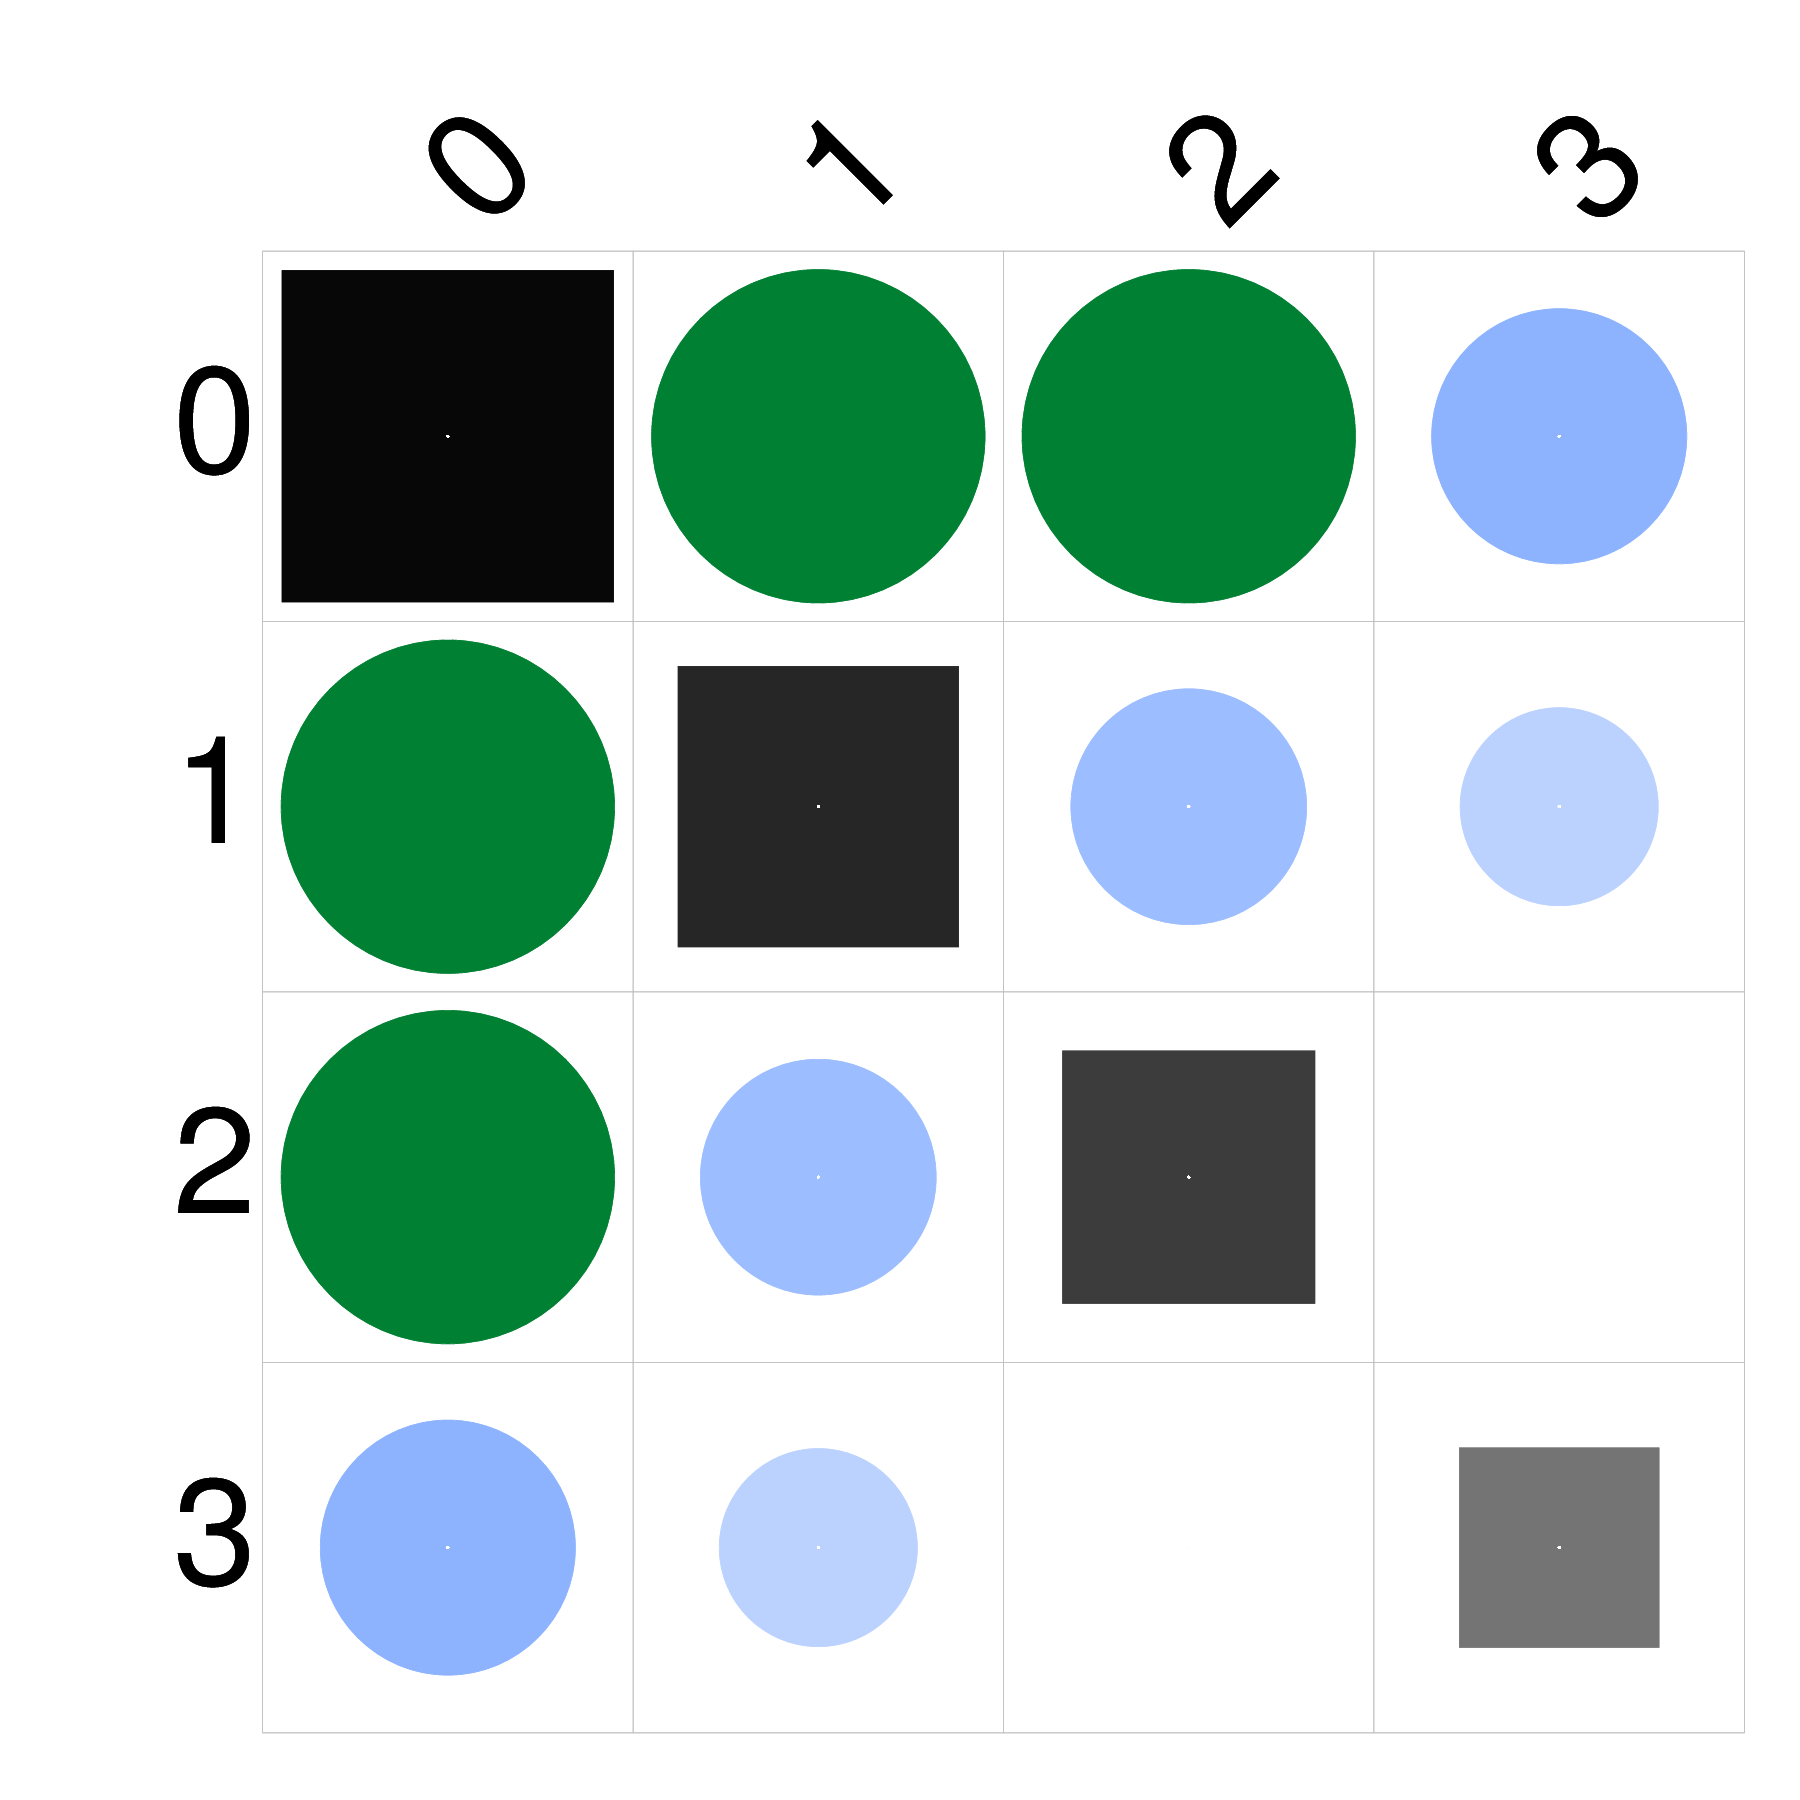
\includegraphics[width=\textwidth]{./images/matrix.png}
    \end{column}
  \end{columns}
  \begin{block}{Complexity measure}\begin{equation*}
      \sqrt{\text{trace}(M^TM)}
  \end{equation*}\end{block}
\end{frame}

\section{Conclusion}

\begin{frame}
  \frametitle{Complete analysis}
  \includegraphics[width=\textwidth]{./images/complete.png}
\end{frame}

\begin{frame}
  \frametitle{Hybrid representation}
  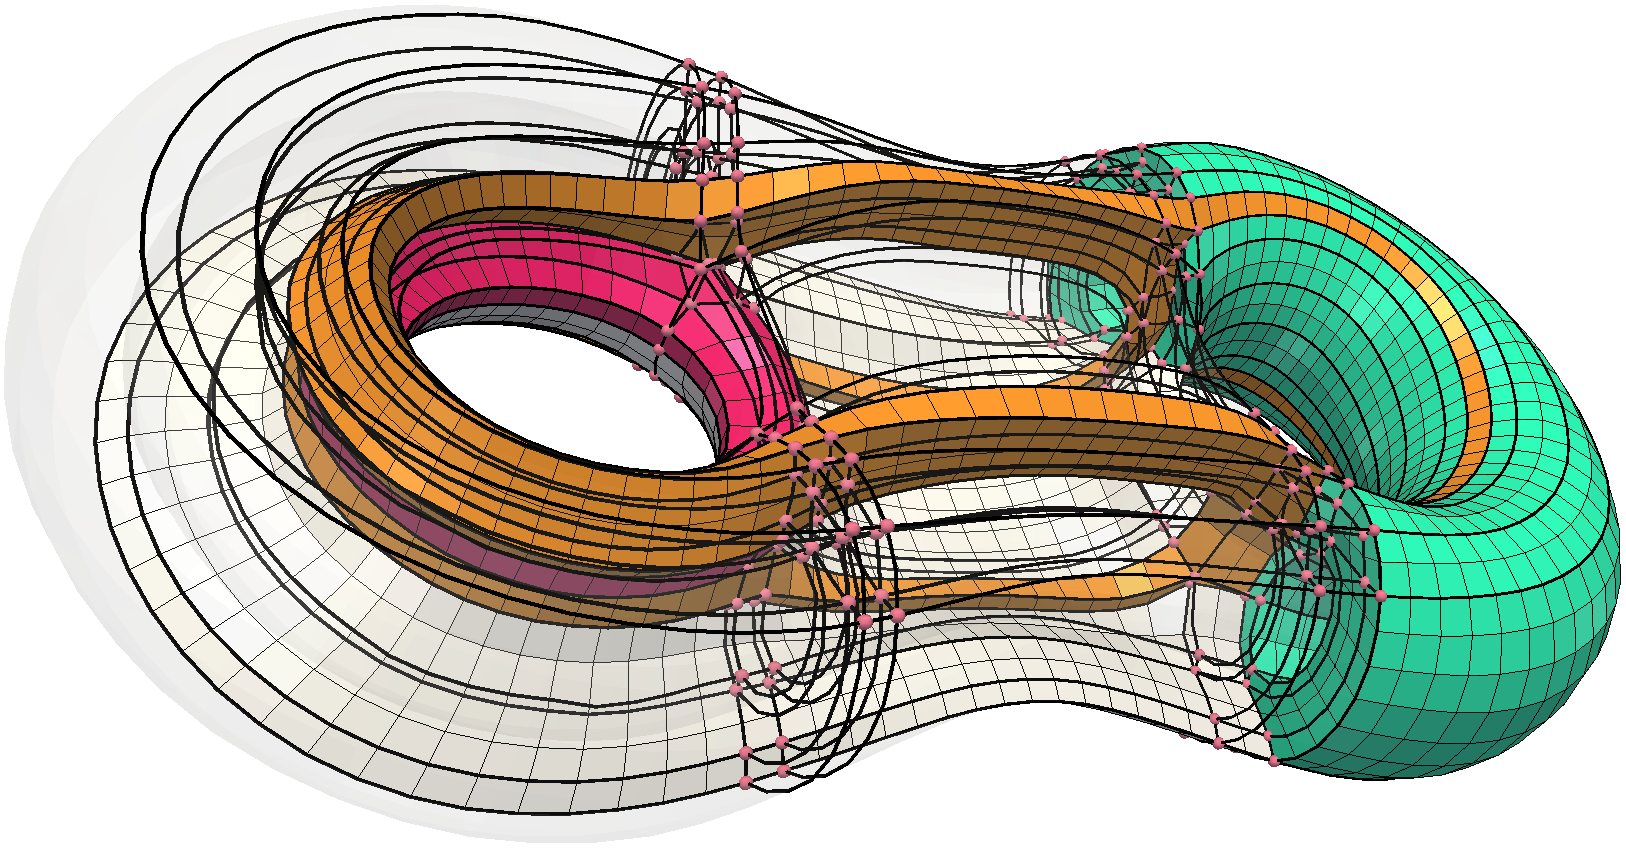
\includegraphics[width=\textwidth]{./images/hybrid.png}
\end{frame}

\end{document}
